\clearpage
\section{Příklady z minulých zkoušek}
\subsection{Zadání 1}
\begin{enumerate}
    \item \textbf{Vypočtěte amplitudu základní(1.) harmonické složky unipolárního signálu RZ při bitové posloupnosti ...101010... Doba trvání impulzu je poloviční oproti době trvání bitu. Výška impulzu je 5V}
    \begin{align*}
        C_1 = 2\cdot D \cdot \frac{\vartheta}{T_0}\cdot sinc(\frac{\vartheta}{2}\cdot\frac{2\pi}{T_0}) = \frac{10}{4} \cdot \frac{sin(\frac{\vartheta}{2}\cdot\frac{2\pi}{4\vartheta})}{\frac{\vartheta}{2}\cdot\frac{2\pi}{4\vartheta}} =  2,2508V
    \end{align*}
    \item \textbf{Jakou minimální kmitočtovou šířku pásma propustnosti potřebuje pro přenos signálu FSK, je-li \(f_1 = 100 kHz\), \(f_0 = 105 kHz\) a data mají být přenášena rychlostí R=5kbit/s.}
    \begin{align*}
        B_{min} = \left | f_0 - f_1 \right | + M \\
        B_{min} = \left | f_0 - f_1 \right | + R \\ 
        B_{min} = 10kHz
    \end{align*}
    V tomto případě se M = R. 
    
    \item \textbf{Blokové schéma modulátoru QPSK}
    \begin{figure}[h]
        \centering
        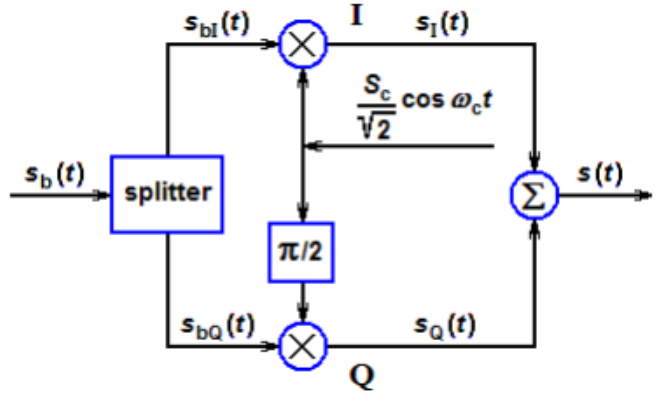
\includegraphics[scale = 0.5]{images/QPSK.png}
        \caption{Modulátor}
    \end{figure}
    \item \textbf{Je dán modulátor 256QAM. Kolika stavový signál je v kanálu I a v kanálu Q?}\
    \begin{align*}
        L_I = L_Q = \sqrt{Q} = \sqrt{256} = 16
    \end{align*}
    Počet stavů signálu v kanálu Q a I je 16
    \item \textbf{Bipolární signál NRZ s napěťovými úrovněmi +5V a -5V je zarušen normálním šumem s
    efektivní hodnotou napětí 1,5V. Pravděpodobnost výskytu log. nuly a jedničky jsou stejné.
    Stanovte pravděpodobnost \(P_E\) chybného příjmu.}
    \begin{align*}
        P_E = F_0(\frac{D_0 - D_1}{2\sigma}) = F_0(-3,33) = 4.3423\cdot10^{-4}
    \end{align*}
    \item \textbf{Nakreslete časový průběh bipolárního signálu NRZ vyjadřujícího dat. posloupnost 10110 a
    odpovídající odezvu přizpůsobeného filtru.}
    \begin{figure}[h]
        \centering
        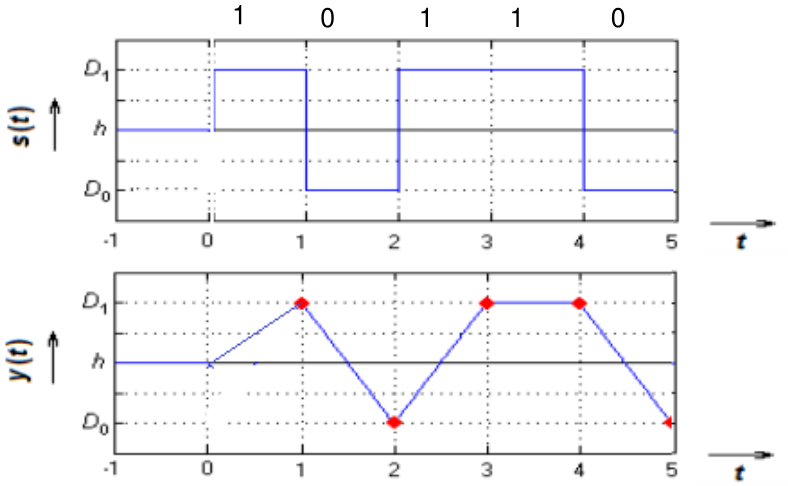
\includegraphics[scale = 0.5]{images/NRZfiltr.png}
        \caption{Průběh a odezva}
    \end{figure}
    \item \textbf{Jaký je účel interleavingu (prokládání), v čem spočívá jeho princip, jakým negativním jevem
    je provázen?}
    \begin{itemize}
        \item Ochrana proti chybám zapříčiněných opakovanými stejnými znaky (0000000000, 1111111) a
        vznikajícími přenosem kanálem.
        \item Jednotlivé bity jsou po výstupu z kodéru pro dopředné potlačení chyb zpožděny o různý čas.
        \item Shluk chyb je rozprostřen, izolované chyby lze opravit.
    \end{itemize}
    \item \textbf{Jak závisí index kmitočtové modulace \(\beta\) na kmitočtu modulačního signálu F a
    kmitočtovém zvdihu \(\Delta f\)?}
    \begin{align*}
        \beta = \frac{\Delta f}{F}
    \end{align*}
    \item \textbf{Signál v základním pásmu je tvořen signálovými prvky linkového kódu 2B1Q s dobou
    trvání \(T_s = 250 \mu s\). Stanovte přenosovou rychlost R a modulační rychlost M.}
    \begin{align*}
        M = \frac{1}{T_s} = \frac{1}{250 \cdot 10^{-6}} = 4kBd\\
        M = \frac{R}{2} \Rightarrow R = 2\cdot M = 8kbit/s
    \end{align*}
    \item \textbf{Do připraveného grafu zakreslete modulové kmit. charakteristiky Nyquistova filtru (raised
    cosine filter) pro následující hodnoty činitele tvaru (roll off factor) \(\alpha = 0, \alpha = 0,5, \alpha = 1\)}
    \begin{figure}[h]
        \centering
        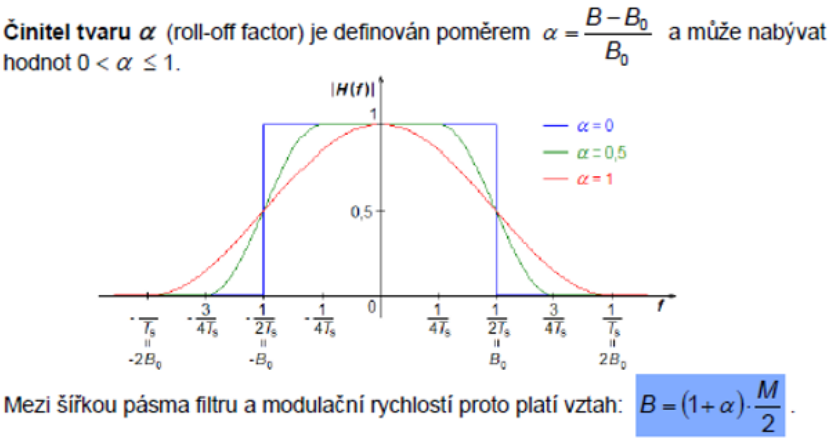
\includegraphics[scale = 0.5]{images/NyquistFilter.png}
        \caption{Nyquistův filter}
    \end{figure}
\end{enumerate}

\subsection{Zadání 2}

\begin{enumerate}
    \item \textbf{Jaký musí být minimální vzorkovací kmitočet kodéru delta modulace, aby nedošlo k jeho
    přetížení, je-li maximální strmost modulačního signálu max [f`(t)] = 800V/s a kvantizační
    krok \(\Delta s = 40mV\)?}
    \begin{align*}
        f_{vz} = \frac{A}{\Delta s} = \frac{800}{0,04} = 20kHz
    \end{align*}
    \item \textbf{Jaký druh klíčování realizuje modulátor na následujícím obrázku? O kolik stupňů nebo
    radiánů se může měnit počáteční fáze takto klíčovaného signálu na rozhraní sousedních
    sign. prvků? Pozn. uvést všechny možné hodnoty.}\\
    \begin{figure}[h]
        \centering
        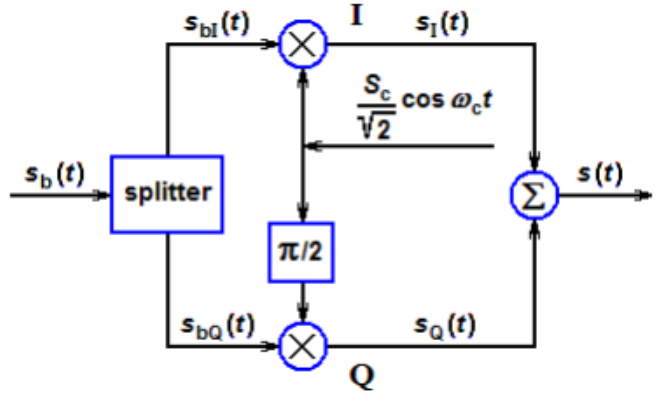
\includegraphics[scale = 0.3]{images/QPSK}
        \caption{Modulátor}
    \end{figure}\\
    Je to QPSK. Počáteční fáze na rozhraní sousedních signálových prvků se mohou měnit o \(\pm \frac{pi}{2} = \pm 90^{\circ}\).
    \item \textbf{Nakreslete časový průběh bipolárního NRZ vyjadřujícího datovou posloupnost 10110 a
    odpovídající odezvu vybíjeného integrátoru.}
    \begin{figure}[h]
        \centering
        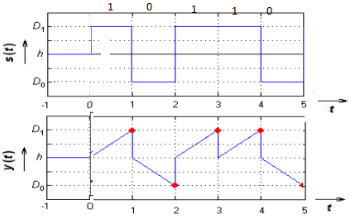
\includegraphics[scale = 0.7]{images/VybInteg.png}
        \caption{Průběh a odezva}
    \end{figure}
    \item \textbf{Je dán kvadraturní modulátor MQAM. Kanál I má 8 stavů, kanál Q má také 8 stavů. Kolik
    bitů vyjadřuje jeden signálový prvek výsledného modulovaného signálu na výstupu modulátoru.}
    \begin{align*}
        M-QAM \Rightarrow M = I\cdot Q = 64\\
        N = log_{2}(M) = log_{2}(64) = 6
    \end{align*}
    \item \textbf{Jaká je hlavní nevýhoda systému DPCM?}\\
    Kumulace chyb
    \item \textbf{Modulovaný signál je popsán rovnicí \(s(t) = S_c cos(\omega_c \cdot t+ \varphi\cdot f(t))\), kde \(f(t)\) je normovaný modulační signál. O jaký druh modulace se jedná? Co vyjadřuje konstanta \(\Delta \varphi\)?}\\
    Jde o fázovou modulaci PM. Kde \(\Delta \varphi\) vyjadřuje fázový zdvih.
    \item \textbf{Kapacita binárního kanálu je C = 0,6 Sh/znak. Stanovte kapacitu C' (maximum vzájemné
    informace přenesené za jednotku času), je-li horní mezní kmitočet kanálu chápaného jako
    dolní propust \(f_h = 500Hz\)}
    \begin{align*}
        C' = 2 \cdot f_h \cdot C = 600Sh/s
    \end{align*}
    \item \textbf{Nakreslete blokové schéma modulátoru sigma–delta}
    \begin{figure}[h]
        \centering
        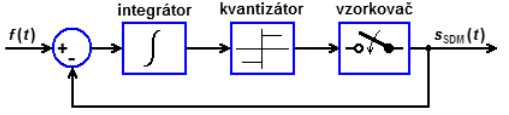
\includegraphics[scale = 0.7]{images/SDM.png}
        \caption{Sigma-Delta modulátor}
    \end{figure}
    \item \textbf{Bipolárním signálem RZ o napěťových úrovních +1V a -1V je přenášena periodická datová
    posloupnost 110110110 Doba trvání impulzu \(\vartheta\) je poloviční oproti trvání bitu,
    která je \(T_b = 250 \mu s\). Určete ss složku signálu a přenosovou rychlost.}
    \begin{align*}
        A_0 = D\cdot\frac{p\vartheta - n\vartheta}{T_0} = 1\frac{1}{6} = 0,1667V\\
        M = \frac{1}{T_s} = 8kBd = 2\cdot R \Rightarrow R = \frac{M}{2} = 4kbit/s
    \end{align*}
    \item \textbf{Do připraveného grafu zakreslete spektrum amplitud signálu BPSK, který přenáší
    periodickou datovou posloupnost 010101. Rychlostí 10kbit/s. Amplituda nosného signálu je
    \(S_c=1V\) a kmitočet \(f_c = 30kHz\).}\\
    \(M = R \Rightarrow B_{min} = M = 10kHz \Rightarrow F = \frac{M}{2} = 5kHz\). Rozestupy mezi harmonickými budou 5kHz.\\
    \begin{figure}[h]
        \centering
        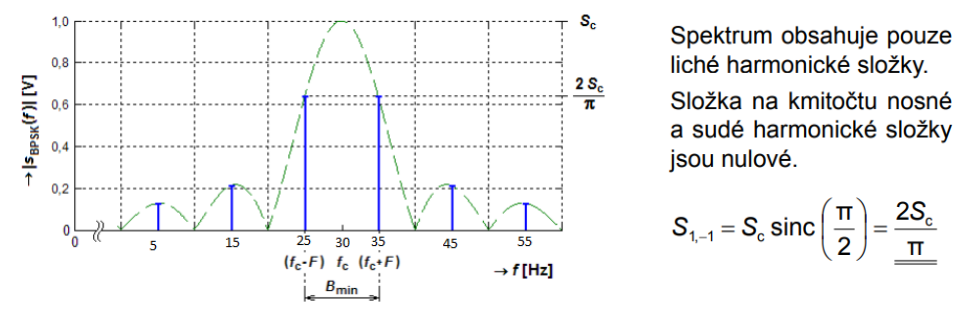
\includegraphics[scale = 0.4]{images/BPSK.png}
        \caption{Spektrum BPSK}
    \end{figure}
\end{enumerate}

\subsection{Zadání 3}
\begin{enumerate}
    \item \textbf{Je dána amplitudová modulace DSB-SC. Klidová amplituda nosné je 5V, hloubka modulace
    je \(30\%\). Kmitočet harmonického modulačního signálu je 1kHz, kmitočet nosné je 1MHz.
    Modulovaný signál působí na zátěž 50 ohmů. Vypočtěte výkon modulovaného signálu na
    této zátěži.}
    \begin{align*}
        P = 2P_s = 2\cdot\frac{(\frac{S_s}{\sqrt{2}})^2}{R} = 2\cdot\frac{\frac{m^2\cdot S_c^2}{8}}{r} = 2\cdot\frac{m^2\cdot S_c^2}{8R} = 11,25mV
    \end{align*}
    \item \textbf{Data jsou přenášena rychlostí 9,6 kbps. Jaká je modulační rychlost je-li použit linkový kód
    4B3T?}
    \begin{align*}
        M = \frac{3}{4}R = 7,2kBd
    \end{align*}
    \item \textbf{Určete amplitudu harmonické složky s kmitočtem 10,002 MHz kmitočtově modulovaného
    signálu. Kmitočtový zdvih je 6 kHz, kmitočet nosné je 10MHz, amplituda nosné je 2V a
    modulační signál je \(f(t)=cos(2\pi\cdot 2\cdot10^3)\cdot t + \varphi\)}
    \begin{gather*}
        F = 2kHz\\
        \beta = \frac{\Delta f}{F} = 3\\
        n = \frac{f_n - f_c}{F} = \frac{10,002\cdot10^6 - 10\cdot10^6}{2\cdot10^3} = 1\\
        S_1 = S_c \left |J_1(\beta) \right | = 0,66V
    \end{gather*}
    \item \textbf{Nakreslete blokové schéma demodulátoru QPSK}\\
    Zadání 1 otázka 3
    \item \textbf{Čím lze kompenzovat aperturové zkreslení u PAM II ?}\\
    Volit kratší vzorkovací periodu a vzorkovat tak častěji než je teoreticky nutné nebo před D/A převodem signál převzorkovat.
    \item \textbf{Je dán kvadraturní modulátor MQAM. Kanál I má 8 stavů, kanál Q má také 8 stavů. Kolik
    bitů vyjadřuje jeden sign. prvek výsledného modulovaného signálu na výstupu modulátoru.}\\
    Zadání 2 otázka 4
    \newpage
    \item \textbf{Nakreslete blokové schéma modulátoru delta}
    \begin{figure}[h]
        \centering
        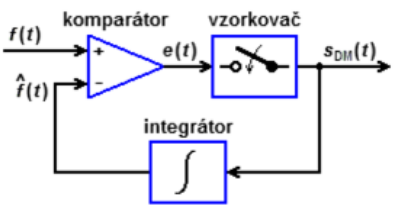
\includegraphics[scale = 0.7]{images/DM.png}
        \caption{Delta modulátor}
    \end{figure}
    \item \textbf{Určete pravděpodobnost chybného příjmu \(P_E\) amplitudově klíčovaného signálu ASK, je-li
    poměr amplitudy nosné a efektivní hodnoty šumu na vstupu součinového (koherentniho)
    demodulátoru \(S_c/\sigma\) = 2,9. Pravděpodobnost výskytu log. 0 a 1 jsou stejné.}
    \begin{gather*}
        P(0)=P(1)=0,5\\
        P_E = F_0(-\frac{1}{2}\cdot\frac{S_c}{\sigma}) = F_0(-1,45) = 7,35\cdot10^{-2}
    \end{gather*}
    \item \textbf{Vyjmenujte čtyři základní metody mnohonásobného přístupu. (Celé názvy, ne jen zkratky)}
    \begin{itemize}
        \item FDMA - frequency division multiple access
        \item TDMA - time division multiple access
        \item CDMA - code division multiple access
        \item ALOHA
    \end{itemize}
    \item \textbf{Jakým druhem klíčování byl vytvořen signál na následujícím obrázku?}\\
    \begin{figure}[h]
        \centering
        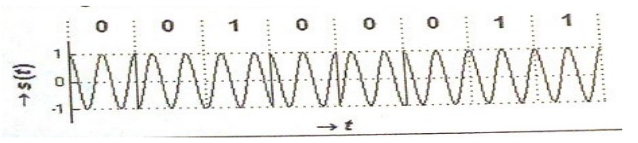
\includegraphics[scale = 0.7]{images/signal.png}
        \caption{Signál}
    \end{figure}\\
    Odpověď: DPSK
\end{enumerate}

\subsection{Zadání 4}
\begin{enumerate}
    \item \textbf{Jaký linkový kód je na nasledujícím obrázku použit k přenosu dat? Stanovte přenosovou
    rychlost R, modulační rychlost M a minimální potřebnou šířku pásma B přenosového
    kanálu, je-li doba trvání signálového prvku \(T_s = 125\mu s\)}\\
    \begin{figure}[h]
        \centering
        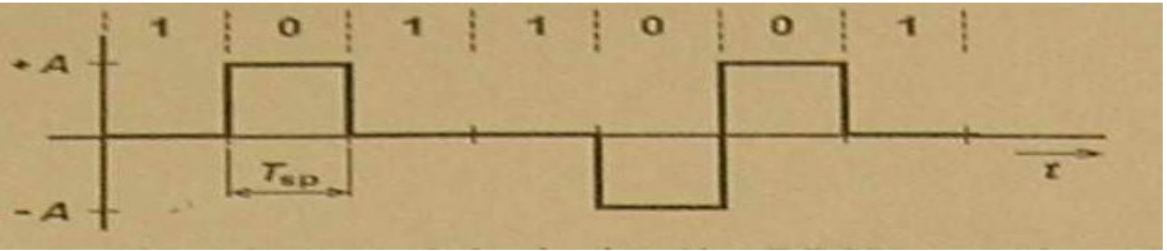
\includegraphics[scale = 0.3]{images/MAMI.png}
        \caption{Linkový kód}
    \end{figure}\\
    Jedná se o kód MAMI.\\
    \(M = \frac{1}{T_s} = 8kBd\) \(R = \frac{1}{T_b} = 8kbit/s\) \(B_{min} = \frac{M}{2} = 4kHz\)
    \item \textbf{Nakreslete blokové schéma a popiste rovnicemi demodulaci signalu BPSK součinovým
    demodulátorem. Pozn. Modulovany signal je popsan rovnici \(s(t)=g(t)\cdot Sc\cdot cos(\omega_c t)\), kde
    g(t) je modulacni signal.}\\
    \begin{figure}[h]
        \centering
        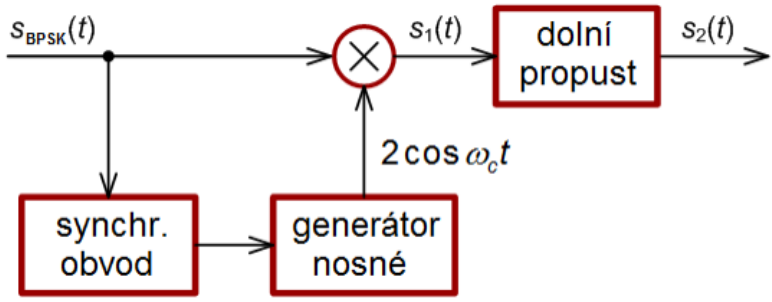
\includegraphics[scale = 0.5]{images/BPSKSchema.png}
        \caption{BPSK schéma}
    \end{figure}\\
    Signál za násobičkou je popsán rovnicí: \(s_1(t) = (S_ccos(\omega_c t)\cdot g(t))\cdot 2cos(\omega_c t) = S_cg(t)\cdot 2cos^2(\omega_c t) = S_cg(t)+S_cg(t)cos(2\omega_ct)\)\\
    Dolní propustí projde pouze signál: \(s_2(t) = S_cg(t)\)
    \item \textbf{Systém OFDM používá 256 nosných. V zakladnim pasmu jsou signalove prvky tvoreny
    modulaci QPSK a mají dobu trvani \(T_s = 32\mu s\). Jaka je celkova prenosova rychlost
    systemu?}
    \begin{gather*}
        M = \frac{1}{T_s} = 31,25kBd\\
        R = Mlog(Q) = 31,25\cdot 10^3 \cdot log_2(4) = 62,5kbit/s\\
        R_{celk} = 256\cdot R = 16Mbit/s
    \end{gather*}
    \item \textbf{Nakreslete blokové schéma detektoru přechodu realizujícího metodu delay-and-multiply a
    časové průběhy vstupního bipolarního NRZ signálu přenášejícího datovou posloupnost
    01001 a odpovídajícího vnitřního a výstupního detektoru.
    }
    \begin{figure}[h]
        \centering
        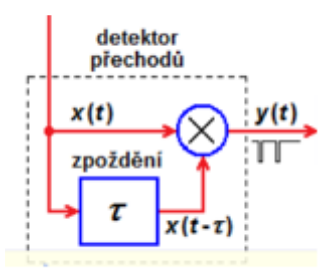
\includegraphics[scale = 0.5]{images/delay-multiply.png}
        \caption{Blokové schéma}
    \end{figure}\\
    \begin{figure}[h]
        \centering
        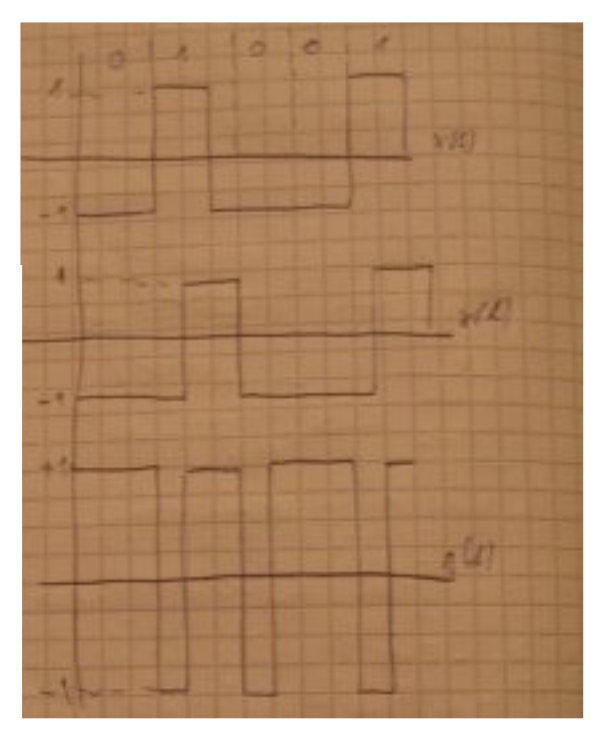
\includegraphics[scale = 0.3]{images/pruběhyDM.png}
        \caption{Průběhy}
    \end{figure}\\
    \item \textbf{Stanovte entropii H a maximalni entropii H0 zdroje zprav produkujiciho posloupnost prvku
    se vzajemne nezavislym vyskytem. Pravdepodobnosti prvku jsou na všech mistech
    posloupnosti tyto: P(A) = 0,1; P(B) = P(C) = P(D) = 0,3}
    \begin{gather*}
        I_a = -log_2(P(A)) = 3,322Sh\\
        I_b = -log_2(P(B)) = 1,737Sh\\
        H = P(A)\cdot I_a + P(B)\cdot 3 \cdot I_b = 1,8936Sh/znak\\
        H_{max} = logN = 2Sh/znak
    \end{gather*}
    
    \item \textbf{Jaká je úloha ekvalizéru? K čemu slouží trénovací posloupnost?}\\
    Ekvalizéry potlačují kmitočtové zkreslení signálu, které vzniká při průchodu sdělovacím kanálem. Trénovací posloupnost se užívá pro nastavení paramterů ekvalizéru.
    \item \textbf{Jaké rozdělení hustoty pravděpodobnosti mají okamžité hodnoty počátečních fází úzkopásmového šumu?}\\
    Rovnoměrné
    \item \textbf{Odhadněte jednoprocentní šířku pásma kmitočtově modulovaného signálu, je-li horní mezní
    kmitočet modulačního signálu \(F_{max} =15 kHz\) a index kmit. modulace \(\beta=5\)}
    \begin{gather*}
        \beta = \frac{\Delta f}{F_{max}} \Rightarrow \Delta f = 75kHz\\
        B = 2\cdot (\Delta f + 3 F_{max}) = 240kHz
    \end{gather*}
    \item \textbf{Uveďte důvod zavedení vztažného klíčování DPSK.}\\
    Odstraňuje problém s fázovou nejistotou.
    \item \textbf{Nakreslete převodní charakteristiku y=f(x) obvodu, jehož odezvy na vstupní harmonický
    signál jsou na následujících obrazcích. Jak se tento obvod (funkční blok) používaný v PCM
    systémech nazývá?}\\
    \begin{figure}[h]
        \centering
        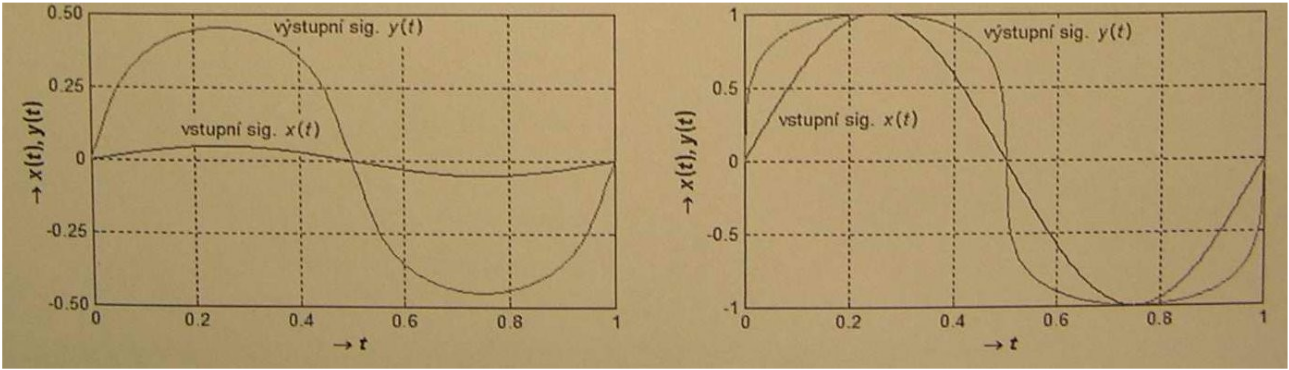
\includegraphics[scale = 0.3]{images/4.10.png}
        \caption{Průběhy}
    \end{figure}\\
    Jedná se o kompresor, malé signály zesiluje a velké nechává stejné.\\
\end{enumerate}

\subsection{Zadání 5}
\begin{enumerate}
    \item \textbf{Je dána amplitudová modulace DSB. Klíčová amplituda nosné je 5V, hloubka modulace je
    30\%. Kmitočet harmonického modulačního signálu je 1 kHz, kmitočet nosné je 1 MHz.
    Modulovaný signál působí na zátěž 50 ohmů. Vypočtěte špičkové napětí modulovaného
    signálu max[s(t)].}
    \begin{gather*}
        m = \frac{\Delta S}{S_c} \Rightarrow \Delta S = m\cdot S_c = 1,5V\\
        S_{max} = S_c + \Delta S = 6,5V
    \end{gather*}
    \item \textbf{Nakreslete blokové schéma skrambleru, který realizuje skramplovací polynom \(P(x) = 1
    \bigoplus  x^2 \bigoplus  x^5\). Jaký je účel použití skrambleru?}\\
    Výsledný signál neobsahuje shluky 0 nebo 1. Např. 00000000 nebo 111111, to umožnuje
    jednodušší synchronizaci v přijímači.\\
    \begin{figure}[h]
        \centering
        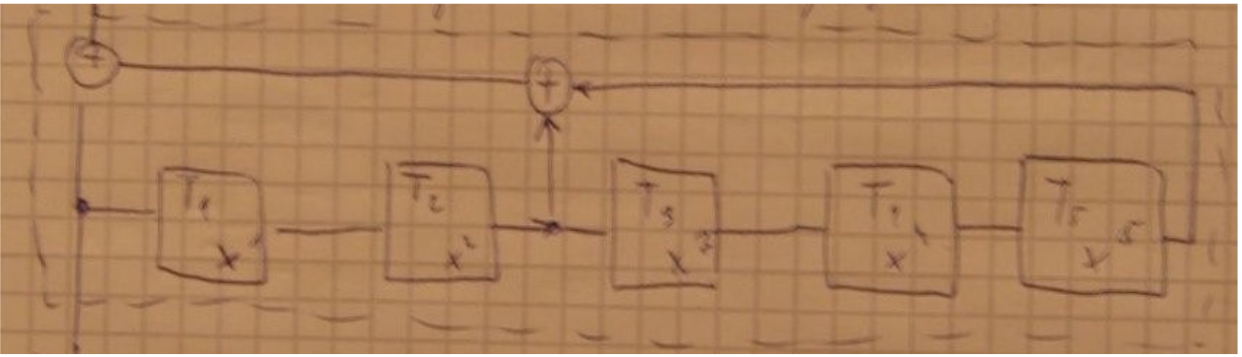
\includegraphics[scale = 0.3]{images/Skrambler.png}
        \caption{Schéma skrambleru}
    \end{figure}\\
    \item \textbf{Signál v základním pásmu je tvořen signálovými prvky linkového kódu 2B1Q s dobou
    trvání \(T_s = 250\mu s\). Stanovte přenosovou rychlost R a modulační rychlost M.}
    \begin{gather*}
        M = \frac{1}{T_s} = 4kBd\\
        M = \frac{R}{2} \Rightarrow R = 2M = 8kbit/s
    \end{gather*}
    \item \textbf{Určete amplitudu harmonického složky s kmitočtem 10,003 MHz fázově modulovaného
    signálu. Fázový zdvih je 5rad. kmitočet nosné je 10MHz. amplituda nosné je 5V. Modulační
    signál je \(f(t) = sin(2\pi \cdot 103t)\) [V]}
    \begin{gather*}
        n = \frac{f_n - f_c}{F_{max}} = \frac{10,003\cdot 10^6 - 10\cdot 10^6}{10^3} = 3\\
        S_3 = S_c \left | J_3(\beta) \right | = 5\cdot \left | J_3(5) \right | = 0,68V
    \end{gather*}
    \item \textbf{Jistý druh modulace je popsán rovnicí \(s(t) = \sum_{n = -\infty}^{\infty} \sum_{m=0}^{M-1}a_{m,n}x_{m,n}\).Co udává proměnná
    M?}\\
    Jedná se o modulaci OFDM a M udává počet nosných.
    \item \textbf{Zakreslete blokové schéma modulátoru MSK. Jaký musí být úhlový kmitočet omegar
    tvarovacího harmonického signálu, je-li přenosová rychlost na vstupu modulátoru 64 kbps}
    \begin{figure}[h]
        \centering
        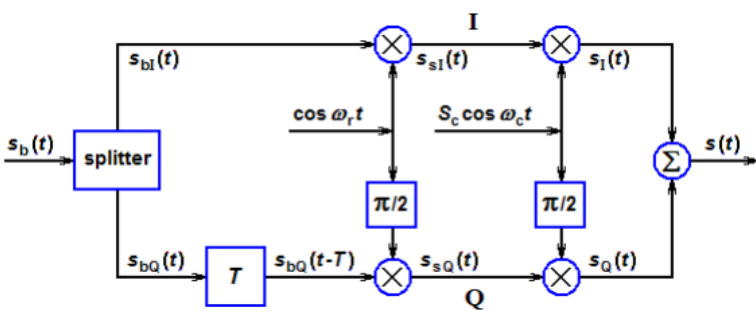
\includegraphics[scale = 0.3]{images/MSK.png}
        \caption{Schéma MSK}
    \end{figure}\\
    \item \textbf{Určete pradvěpodobnost chybného příjmu signálu DPSK, je li poměr amplitudy nosné a
    efektivní hodnoty šumu na vstupu součinového tj. koherentního demodulátoru \(S_c/\sigma
    =-2,9\)}
    \begin{gather*}
        P_E = 2F_0(\frac{-S_c}{\sigma}) = 2F_0(-2,9) = 3,72\cdot 10^{-2}
    \end{gather*}
    \item \textbf{Jaký druh modulace odpovídá následujícímu obrázku?}\\
    \begin{figure}[h]
        \centering
        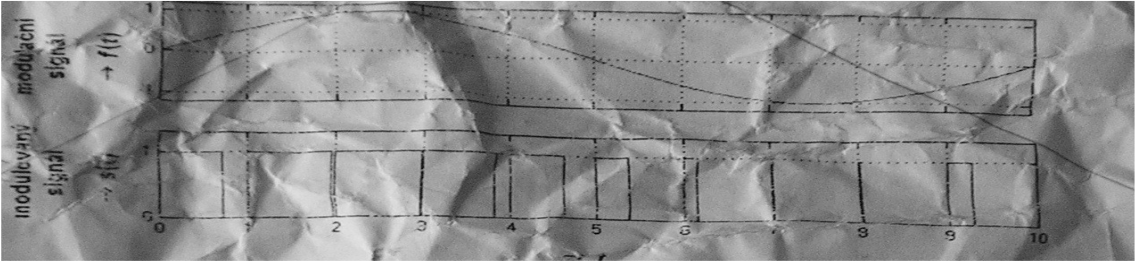
\includegraphics[scale = 0.3]{images/PWMAsy.png}
        \caption{Zadání}
    \end{figure}\\
    Je to šířková impulsová asymetrická modulace.
    \item \textbf{V osách 1 a O nakreslete vektorový diagram modulace QPSK. Vyznačte všechny možné
    přechody mezi po sobě jdoucími symboly.}
    \begin{figure}[h]
        \centering
        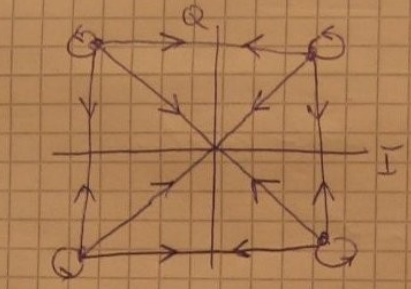
\includegraphics[scale = 0.5]{images/QPSKMal.png}
        \caption{QPSK}
    \end{figure}\\
    \item \textbf{Jak je definována hloubka amplitudové modulace a jakých hodnot nabývá?}\\
    Nabývá hodnot od 0 do 1 a je definována jako poměr amplitudového zdvihu a amplitudy nosné
\end{enumerate}

\subsection{Zadání 6}
\begin{enumerate}
    \item \textbf{Je dána modulace 64QAM. Doba trvání signálového prvku modulovaného signálu je \(1\mu s\). Jaká je přenosová rychlost?}
    \begin{gather*}
        M = \frac{1}{T_s} = \frac{1}{10^{-6}} = 1MBd\\
        R = Mlog_2(Q) = 10^6log_2(64) = 6Mbit/s
    \end{gather*}
    \item \textbf{Modulačním signalem je řečový signál dislokovaný v kmit. pásmu od 300Hz do 3400 Hz.
    Určete šířku spektra signálu SSB–SC.}
    \begin{gather*}
        B = f_{max} - f_{min} = 3400 - 300 = 3100Hz
    \end{gather*}
    \item \textbf{Jaké jsou dvě požadované vlastnosti linkových kódů}
    \begin{itemize}
        \item Potlačení SS signálů
        \item Zabránění vzniku dalších úseků s konstantní úrovní
    \end{itemize}
    \item \textbf{Vypočtěte amplitudu základní tj. první harmonické složky unipolárního signálu NRZ při
    přenosu periodické datové poosloupnosti 100100100 výška impulzů je 1V}
    \begin{gather*}
        C_1 = 2D\frac{\vartheta}{T_0}sinc(\frac{\vartheta}{2}\frac{2\pi}{T_0}) = \frac{2}{3}D\cdot \frac{sin(\frac{\pi}{3})}{\frac{\pi}{3}} = 0,55V
    \end{gather*}
    \item \textbf{Nakreslete blokové schéma systému pro obnovu nosné fázově klíčovaného signálu BPSK}
    \begin{figure}[h]
        \centering
        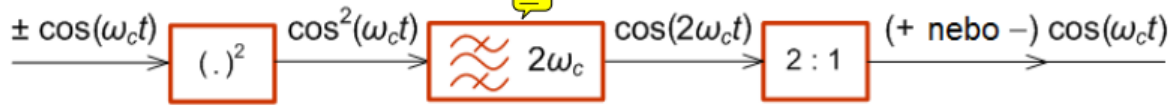
\includegraphics[scale = 0.3]{images/DemodBPSK.png}
        \caption{Schema}
    \end{figure}\\
    \item \textbf{Jakou metodu mnohonásobného přístupu používá vysílač na následujícím obrázku? Co
    udává poměr přenosových rychlostí Rch a Rb?}\\
    \begin{figure}[h]
        \centering
        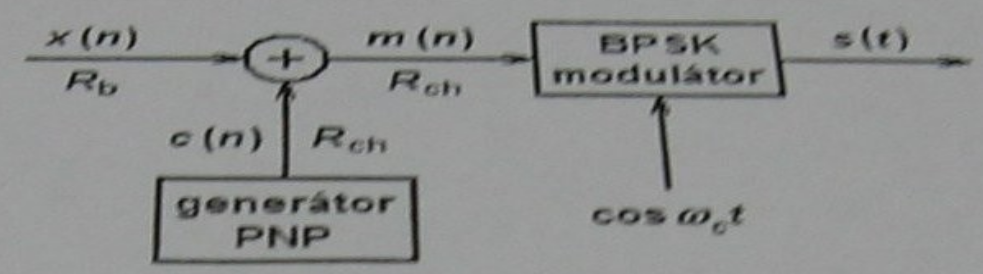
\includegraphics[scale = 0.5]{images/MoDS.png}
        \caption{Schema}
    \end{figure}\\
    Modulátor s přímou modulací kódovu posloupností(DS). Poměr rychlostí udává činitel rozprostření
    \item \textbf{Unipolární signál NRZ s výškou impulzů D=5V je zarušen normálním šumem s efektivní
    hodnotou napětí 1,5V. Pravděpodobnosti výskytu 0 a 1 jsou stejné. Stanovte
    pravděpodobnost Pch chybného příjmu.}
    \begin{gather*}
        P_E = F_0(\frac{D_0 - D_1}{2\sigma}) = F_0(-1,5) = 0,048
    \end{gather*}
    \item \textbf{Jakou minimální kmitočtovou šířku pásma propustnosti pro přenos signálu ASK. je li
    přenosová rychlost R=64 kbit/s}
    \begin{gather*}
        B_{min} = 2F = M = R = 64kHz
    \end{gather*}
    \item \textbf{Nakreslete převodní charakteristiky y=f(x) kompresoru a expandoru}\\
    \begin{figure}[h]
        \centering
        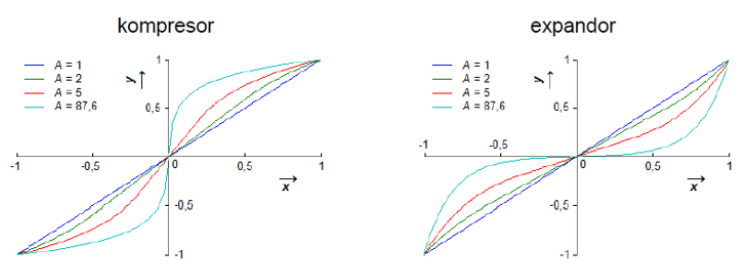
\includegraphics[scale = 0.5]{images/PrevodniCharakteristiky.png}
        \caption{Kompresor expander}
    \end{figure}\\
    \item \textbf{Na vstup součinového (koherentního) demodulátoru působí pouze úzkopásmový šum. Jaké
    je rozdělení hustoty pravděpodobnosti mají okamžité hodnoty šumu na výstupu
    demodulátoru a jaká bude jeho střední hodnota?}\\
    Rovnoměrné
\end{enumerate}
